%-------------------------------------------------------
% SLEPc Users Manual
%-------------------------------------------------------
\chapter{\label{cap:svd}SVD: Singular Value Decomposition}
%-------------------------------------------------------

\noindent The Singular Value Decomposition (\ident{SVD}) solver object can be used for computing a partial SVD of a rectangular matrix, and other related problems. It provides uniform and efficient access to several specific SVD solvers included in \slepc, and also gives the possibility to compute the decomposition via the eigensolvers provided in the \ident{EPS} package.

In many aspects, the user interface of \ident{SVD} resembles that of \ident{EPS}. For this reason, this chapter and chapter \ref{cap:eps} have a very similar structure.
	
\section{\label{sec:svdback}Mathematical Background}

This section provides some basic concepts about the singular value decomposition and other related problems. The objective is to set up the notation and also to justify some of the solution approaches, particularly those based on the \ident{EPS} object. As in the case of eigensolvers, some of the implemented methods are described in detail in the \slepc \hyperlink{str}{technical reports}.

For background material about the SVD, see for instance \citep[ch.~6]{Bai:2000:TSA}. Many other books such as \citep{Bjorck:1996:NML} or \citep{Hansen:1998:RDI} present the SVD from the perspective of its application to the solution of least squares problems and other related linear algebra problems.

\subsection{\label{sec:svd}The (Standard) Singular Value Decomposition (SVD)}

The singular value decomposition (SVD) of an $m\times n$ matrix $A$ can be written as
\begin{equation}
\label{eq:svd}
A=U\Sigma V^*,
\end{equation}
where $U=[u_1,\ldots,u_m]$ is an $m\times m$ unitary matrix ($U^*U=I$), $V=[v_1,\ldots,v_n]$ is an $n\times n$ unitary matrix ($V^*V=I$), and $\Sigma$ is an $m\times n$ diagonal matrix with real diagonal entries $\Sigma_{ii}=\sigma_i$ for $i=1,\ldots,\min\{m,n\}$. If $A$ is real, $U$ and $V$ are real and orthogonal. The vectors $u_i$ are called the left singular vectors, the $v_i$ are the right singular vectors, and the $\sigma_i$ are the singular values.

\begin{figure}
\centering
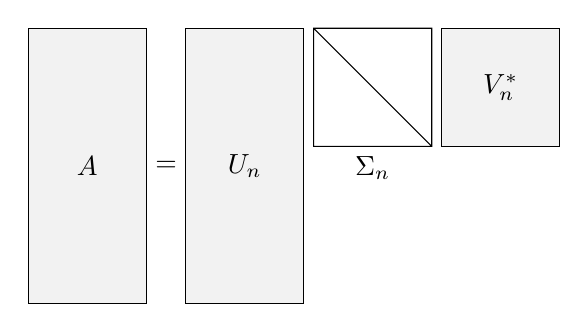
\begin{tikzpicture}[scale=0.5]
  \draw[fill=black!5] (0,0) rectangle node {$A$} +(3,7);
  \node at (3.5,3.5) {=};
  \draw[fill=black!5] (4,0) rectangle node {$U_n$} +(3,7);
  \draw (7.25,4) rectangle +(3,3) (7.25,7) -- +(3,-3);
  \node[below] at (8.75,4) {$\Sigma_n$};
  \draw[fill=black!5] (10.5,4) rectangle node {$V_n^*$} +(3,3);
\end{tikzpicture}
\caption{\label{fig:svd}Scheme of the thin SVD of a rectangular matrix $A$.}
\end{figure}

In the following, we will assume that $m\geq n$. If $m<n$ then $A$ should be replaced by $A^*$ (note that in \slepc this is done transparently as described later in this chapter and the user need not worry about this). In the case that $m\geq n$, the top $n$ rows of $\Sigma$ contain $\mathrm{diag}(\sigma_1,\ldots,\sigma_n)$ and its bottom $m-n$ rows are zero. The relation \eqref{eq:svd} may also be written as $AV=U\Sigma$, or
\begin{equation}
\label{eq:svdleft}
Av_i=u_i\sigma_i\;,\quad i=1,\ldots,n,
\end{equation}
and also as $A^*U=V\Sigma^*$, or
\begin{align}
\label{eq:svdright}
A^*u_i&=v_i\sigma_i\;,\quad i=1,\ldots,n,\\
\label{eq:svdright2}
A^*u_i&=0\;,\quad i=n+1,\ldots,m.
\end{align}
The last left singular vectors corresponding to \eqref{eq:svdright2} are often not computed, especially if $m\gg n$. In that case, the resulting factorization is sometimes called the \emph{thin} SVD, $A=U_n\Sigma_n V_n^*$, and is depicted in Figure \ref{fig:svd}. This factorization can also be written as
\begin{equation}
\label{eq:svdouter}
A=\sum_{i=1}^{n}\sigma_iu_iv_i^*.
\end{equation}
Each $(\sigma_i,u_i,v_i)$ is called a singular triplet.

The singular values are real and nonnegative, $\sigma_1\geq\sigma_2\geq\ldots\geq\sigma_r>\sigma_{r+1}=\ldots=\sigma_n=0$, where $r=\mathrm{rank}(A)$. It can be shown that $\{u_1,\ldots,u_r\}$ span the range of $A$, $\mathcal{R}(A)$, whereas $\{v_{r+1},\ldots,v_n\}$ span the null space of $A$, $\mathcal{N}(A)$.

If the zero singular values are dropped from the sum in \eqref{eq:svdouter}, the resulting factorization, $A=\sum_{i=1}^{r}\sigma_iu_iv_i^*$, is called the \emph{compact} SVD, $A=U_r\Sigma_r V_r^*$.

In the case of a very large and sparse $A$, it is usual to compute only a subset of $k\leq r$ singular triplets. We will refer to this decomposition as the \emph{truncated} SVD of $A$. It can be shown that the matrix $A_k=U_k\Sigma_k V_k^*$ is the best rank-$k$ approximation to matrix $A$, in the least squares sense.

In general, one can take an arbitrary subset of the summands in \eqref{eq:svdouter}, and the resulting factorization is called the \emph{partial} SVD of $A$. As described later in this chapter, \slepc allows the computation of a partial SVD corresponding to either the $k$ largest or smallest singular triplets.

\paragraph{Equivalent Eigenvalue Problems.}

It is possible to formulate the problem of computing the singular triplets of a matrix $A$ as an eigenvalue problem involving a Hermitian matrix related to $A$. There are two possible ways of achieving this:
\begin{enumerate}
\item With the \emph{cross product} matrix, either $A^*A$ or $AA^*$.
\item With the \emph{cyclic} matrix, $H(A)=\left[\begin{smallmatrix}0&A\\A^*&0\end{smallmatrix}\right]$.
\end{enumerate}
In \slepc, the computation of the SVD is usually based on one of these two alternatives, either by passing one of these matrices to an \ident{EPS} object or by performing the computation implicitly.

By pre-multiplying \eqref{eq:svdleft} by $A^*$ and then using \eqref{eq:svdright}, the following relation results
\begin{equation}
\label{eq:eigleft}
A^*Av_i=\sigma_i^2v_i,
\end{equation}
that is, the $v_i$ are the eigenvectors of matrix $A^*A$ with corresponding eigenvalues equal to $\sigma_i^2$. Note that after computing $v_i$ the corresponding left singular vector, $u_i$, is readily available through \eqref{eq:svdleft} with just a matrix-vector product, $u_i=\frac{1}{\sigma_i}Av_i$.

Alternatively, one could first compute the left vectors and then the right ones. For this, pre-multiply \eqref{eq:svdright} by $A$ and then use \eqref{eq:svdleft} to get
\begin{equation}
\label{eq:eigright}
AA^*u_i=\sigma_i^2u_i.
\end{equation}
In this case, the right singular vectors are obtained as $v_i=\frac{1}{\sigma_i}A^*u_i$.

The two approaches represented in \eqref{eq:eigleft} and \eqref{eq:eigright} are very similar. Note however that $A^*A$ is a square matrix of order $n$ whereas $AA^*$ is of order $m$. In cases where $m\gg n$, the computational effort will favor the $A^*A$ approach. On the other hand, the eigenproblem \eqref{eq:eigleft} has $n-r$ zero eigenvalues and the eigenproblem \eqref{eq:eigright} has $m-r$ zero eigenvalues. Therefore, continuing with the assumption that $m\geq n$, even in the full rank case the $AA^*$ approach may have a large null space resulting in difficulties if the smallest singular values are sought. In \slepc, this will be referred to as the cross product approach and will use whichever matrix is smaller, either $A^*A$ or $AA^*$.

Computing the SVD via the cross product approach may be adequate for determining the largest singular triplets of $A$, but the loss of accuracy can be severe for the smallest singular triplets. The cyclic matrix approach is an alternative that avoids this problem, but at the expense of significantly increasing the cost of the computation. Consider the eigendecomposition of
\begin{equation}
\label{eq:cyclic}
H(A)=\begin{bmatrix}0&A\\A^*&0\end{bmatrix},
\end{equation}
which is a Hermitian matrix of order $(m+n)$. It can be shown that $\pm\sigma_i$ is a pair of eigenvalues of $H(A)$ for $i=1,\ldots,r$ and the other $m+n-2r$ eigenvalues are zero. The unit eigenvectors associated with $\pm\sigma_i$ are $\frac{1}{\sqrt{2}}\left[\begin{smallmatrix}\pm u_i\\v_i\end{smallmatrix}\right]$. Thus it is possible to extract the singular values and the left and right singular vectors of $A$ directly from the eigenvalues and eigenvectors of $H(A)$. Note that in this case the singular values are not squared, and therefore the computed values will be more accurate (especially the small ones). The drawback in this case is that small eigenvalues are located in the interior of the spectrum.

\subsection{\label{sec:gsvd}The Generalized Singular Value Decomposition (GSVD)}

An extension of the SVD to the case of two matrices is the generalized singular value decomposition (GSVD), which can be applied in constrained least squares problems, among others. An overview of the problem can be found in~\citep[\S 8.7.3]{Golub:1996:MC}.

Consider two matrices, $A\in\mathbb{C}^{m\times n}$ with $m\geq n$ and $B\in\mathbb{C}^{p\times n}$. Note that both matrices must have the same column dimension. Then there exist two unitary matrices $U\in\mathbb{C}^{m\times m}$ and $V\in\mathbb{C}^{p\times p}$ and an invertible matrix $X\in\mathbb{C}^{n\times n}$ such that
\begin{equation}
\label{eq:gsvd}
U^*AX=C,\qquad V^*BX=S,
\end{equation}
where $C=\mathrm{diag}(c_1,\dots,c_n)$ and $S=\mathrm{diag}(s_{n-q+1},\dots,s_n)$ with $q=\min(p,n)$. The values $c_i$ and $s_i$ are real and nonnegative, and the ratios define the generalized singular values,
\begin{equation}
\label{eq:gsvd-values}
\sigma(A,B)\equiv\{c_1/s_1,\dots,c_q/s_q\},
\end{equation}
and if $p<n$ we can consider that the first $n-p$ generalized singular values are infinite, as if $s_1=\dots=s_{n-p}=0$. Note that if $B$ is the identity matrix, $X$ can be taken to be unitary and then we recover the standard SVD, $\sigma(A,I)=\sigma(A)$, that is why \eqref{eq:gsvd} is considered a generalization of the SVD.

The diagonal matrices $C$ and $S$ satisfy $C^*C+S^*S=I$, and are related to the CS decomposition~\citep[\S 2.6.4]{Golub:1996:MC} associated with the orthogonal factor of the QR factorization of matrices $A$ and $B$ stacked, that is, if
\begin{equation}
\label{eq:qr}
Z:=\begin{bmatrix}A\\B\end{bmatrix}=\begin{bmatrix}Q_1\\Q_2\end{bmatrix}R,
\end{equation}
then $C$ and $S$ can be obtained from the singular values of $Q_1$ and $Q_2$, respectively. The matrix $Z$ is relevant for algorithms and is often built explicitly.

\begin{figure}
\centering
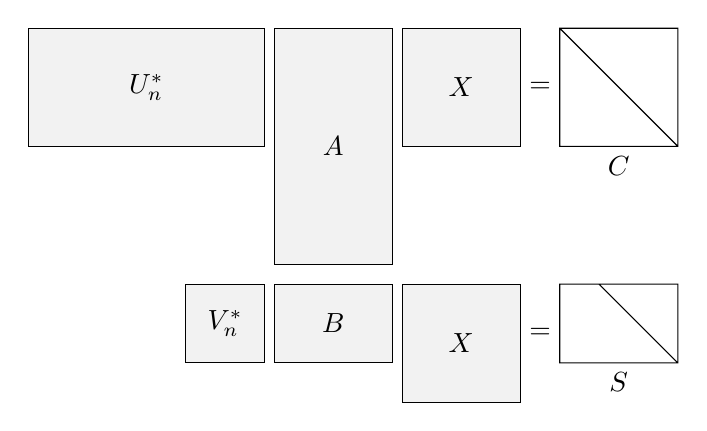
\begin{tikzpicture}[scale=0.5]
  \draw[fill=black!5] (-6.25,3) rectangle node {$U_n^*$} +(6,3);
  \draw[fill=black!5] (0,0) rectangle node {$A$} +(3,6);
  \draw[fill=black!5] (3.25,3) rectangle node {$X$} +(3,3);
  \node at (6.75,4.5) {=};
  \draw (7.25,3) rectangle +(3,3) (7.25,6) -- +(3,-3);
  \node[below] at (8.75,3) {$C$};
  \begin{scope}[yshift=-3.5cm]
  \draw[fill=black!5] (-2.25,1) rectangle node {$V_n^*$} +(2,2);
  \draw[fill=black!5] (0,1) rectangle node {$B$} +(3,2);
  \draw[fill=black!5] (3.25,0) rectangle node {$X$} +(3,3);
  \node at (6.75,1.75) {=};
  \draw (7.25,1) rectangle +(3,2) ++(3,0) -- +(-2,2);
  \node[below] at (8.75,1) {$S$};
  \end{scope}
\end{tikzpicture}
\caption{\label{fig:gsvd}Scheme of the thin GSVD of two matrices $A$ and $B$, for the case $p<n$.}
\end{figure}

The above description assumes that matrix $Z$ has full column rank, and the rank of $B$ is also $q$. In the general case where these assumptions do not hold, the structure of matrices $C$ and $S$ is a bit more complicated. This includes also the case where $m<n$. A detailed description of those cases can be found in~\citep[\S 2.3.5.3]{Anderson:1999:LUG}.

As in the case of the SVD, one can consider thin, compact, truncated, and partial versions of the GSVD. A pictorial representation of the thin GSVD is shown in Figure \ref{fig:gsvd}.

The columns of $X$, $x_i$, are called the (right) generalized singular vectors. The left vectors in this case would correspond to the columns of $U$ and $V$. In SLEPc, the user interface will provide these vectors stacked on top of each other, as a single $(m+p)$-vector $\begin{bmatrix}u_i\\v_i\end{bmatrix}$.

\paragraph{Equivalent Eigenvalue Problems.}
In the GSVD it is also possible to formulate the problem as an eigenvalue problem, which opens the door to approach its solution via \ident{EPS}. The columns of $X$ satisfy
\begin{equation}
\label{eq:gsvdeigcross}
s_i^2A^*Ax_i=c_i^2B^*Bx_i,
\end{equation}
and so if $s_i\neq 0$ then $A^*Ax_i=\sigma_i^2B^*Bx_i$, a generalized eigenvalue problem for the matrix pair $(A^*A,B^*B)$. This is the analog of the cross product matrix eigenproblem of~\eqref{eq:eigleft}.

The formulation that is analog to the eigenproblem associated with the cyclic matrix~\eqref{eq:cyclic} is to solve the generalized eigenvalue problem defined by any of the matrix pairs
\begin{equation}
\label{eq:gsvdeigcyclic}
\left(
\begin{bmatrix}0&A\\A^*&0\end{bmatrix},
\begin{bmatrix}I&0\\0&B^*B\end{bmatrix}
\right),
\qquad\text{or}\qquad
\left(
\begin{bmatrix}0&B\\B^*&0\end{bmatrix},
\begin{bmatrix}I&0\\0&A^*A\end{bmatrix}
\right).
\end{equation}

\subsection{\label{sec:hsvd}The Hyperbolic Singular Value Decomposition (HSVD)}

The hyperbolic singular value decomposition (HSVD) was introduced in~\citep{Onn:1991:HSV}, motivated by some signal processing applications such as the so-called covariance differencing problem. The formulation of the HSVD is similar to that of the SVD, except that $U$ is orthogonal with respect to a signature matrix,
\begin{equation}
\label{eq:hsvd}
A=U\Sigma V^*,\qquad U^*\Omega U=\tilde\Omega,
\end{equation}
where $\Omega=\mathrm{diag}(\pm 1)$ is an $m\times m$ signature matrix provided by the user, while $\tilde\Omega$ is another signature matrix obtained as part of the solution. Sometimes $U$ is said to be a hyperexchange matrix, or also an $(\Omega,\tilde\Omega)$-orthogonal matrix. Note that in the problem definition normally found in the literature it is $V$ that is $(\Omega,\tilde\Omega)$-orthogonal and not $U$. We choose this definition for consistency with respect to the generalized HSVD of two matrices. If the user wants to compute the HSVD according to the alternative definition, then it suffices to (conjugate) transpose the input matrix $A$, using for instance \ident{MatHermitianTranspose}.

As in the case of the SVD, the solution of the problem consists in singular triplets $(\sigma_i,u_i,v_i)$, with $\sigma_i$ real and nonnegative and sorted in nonincreasing order. Note that these quantities are different from those of \S\ref{sec:svd}, even though we use the same notation here. With each singular triplet, there is an associated sign $\tilde\omega_i$ (either 1 or $-1$), the corresponding diagonal element of $\tilde\Omega$. In SLEPc, this value is not returned by the user interface, but if required it can be easily computed as $u_i^*\Omega u_i$.

The relations between left and right singular vectors are slightly different from those of the standard SVD. We have $AV=U\Sigma$ and $A^*\Omega U=V\Sigma^*\tilde\Omega$, so for $m\geq n$ the following relations hold, together with~\eqref{eq:svdleft}:
\begin{align}
\label{eq:hsvdright}
A^*\Omega u_i&=v_i\sigma_i\tilde\omega_i\;,\quad i=1,\ldots,n,\\
\label{eq:hsvdright2}
A^*\Omega u_i&=0\;,\quad i=n+1,\ldots,m.
\end{align}
In SLEPc we will compute a partial HSVD consisting of either the largest or smallest hyperbolic singular triplets. Note that the sign $\tilde\omega_i$ is not used when sorting for largest or smallest $\sigma_i$.

\paragraph{Equivalent Eigenvalue Problems.}
Once again, we can derive cross and cyclic schemes to compute the decomposition by solving an eigenvalue problem. The cross product matrix approach has two forms, to be selected depending on whether $m\geq n$ or not, as discussed in \S\ref{sec:svd}. The first form,
\begin{equation}
\label{eq:heigleft}
A^*\Omega Av_i=\sigma_i^2\tilde\omega_iv_i,\\
\end{equation}
is derived by pre-multiplying~\eqref{eq:svdleft} by $A^*\Omega$ an then using~\eqref{eq:hsvdright}. This eigenproblem can be solved as a HEP (cf.~\S\ref{sec:defprob}) and may have both positive and negative eigenvalues, corresponding to $\tilde\omega_i=1$ and $\tilde\omega_i=-1$, respectively. Once the right vector $v_i$ has been computed, the corresponding left vector can be obtained using~\eqref{eq:svdleft} with just a matrix-vector product, $u_i=\sigma_i^{-1}Av_i$.

The second form of cross computes the left vectors first, by pre-multiplying~\eqref{eq:hsvdright} by $A$ and then using~\eqref{eq:svdleft},
\begin{equation}
\label{eq:heigright}
AA^*\Omega u_i=\sigma_i^2\tilde\omega_iu_i.
\end{equation}
In this case, the right singular vectors are obtained as $v_i=(\sigma_i\tilde\omega_i)^{-1}A^*\Omega u_i$. The coefficient matrix of~\eqref{eq:heigright} is non-Hermitian, so the eigenproblem has to be solved as non-Hermitian, or alternatively it can be formulated as a generalized eigenvalue problem of GHIEP type (cf.~\S\ref{sec:defprob}) for the indefinite pencil $(AA^*,\Omega)$,
\begin{equation}
\label{eq:heigright2}
AA^*\hat{u}_i=\sigma_i^2\tilde\omega_i\Omega \hat{u}_i,
\end{equation}
with $\hat{u}=\Omega u$. The eigenvectors obtained from~\eqref{eq:heigright} or~\eqref{eq:heigright2} must be normalized so that $U^*\Omega U=\tilde\Omega$ holds.

Finally, in the cyclic matrix approach for the HSVD we must solve a generalized eigenvalue problem defined by the matrices of order $(m+n)$
\begin{equation}
\label{eq:hcyclic}
H(A)=\begin{bmatrix}0&A\\A^*&0\end{bmatrix},\qquad
\hat\Omega=\begin{bmatrix}\Omega&0\\0&I\end{bmatrix}.
\end{equation}
As in the case of~\eqref{eq:heigright2}, this pencil is Hermitian-indefinite and hence it may have complex eigenvalues. However, it can be shown that nonzero eigenvalues of the pencil $(H(A),\hat\Omega)$ are either real (equal to $\pm\sigma_i$ for a certain hyperbolic singular value $\sigma_i$) or purely imaginary (equal to $\pm\sigma_ij$ for a certain $\sigma_i$ with $j=\sqrt{-1}$). The associated eigenvectors are $\left[\begin{smallmatrix}\varsigma_i u_i\\v_i\end{smallmatrix}\right]$, where $\varsigma_i$ is either $\pm 1$ or $\pm j$.

%---------------------------------------------------
\section{Basic Usage}

From the perspective of the user interface, the \ident{SVD} package is very similar to \ident{EPS}, with some differences that will be highlighted shortly.

\begin{figure}
\begin{Verbatim}[fontsize=\small,numbers=left,numbersep=6pt,xleftmargin=15mm]
SVD       svd;       /*  SVD solver context  */
Mat       A;         /*  problem matrix      */
Vec       u, v;      /*  singular vectors    */
PetscReal sigma;     /*  singular value      */
PetscInt  j, nconv;
PetscReal error;

SVDCreate( PETSC_COMM_WORLD, &svd );
SVDSetOperators( svd, A, NULL );
SVDSetProblemType( svd, SVD_STANDARD );
SVDSetFromOptions( svd );
SVDSolve( svd );
SVDGetConverged( svd, &nconv );
for (j=0; j<nconv; j++) {
  SVDGetSingularTriplet( svd, j, &sigma, u, v );
  SVDComputeError( svd, j, SVD_ERROR_RELATIVE, &error );
}
SVDDestroy( &svd );
\end{Verbatim}
\caption{\label{fig:ex-svd}Example code for basic solution with \ident{SVD}.}
\end{figure}

The basic steps for computing a partial SVD with \slepc are illustrated in Figure \ref{fig:ex-svd}. The steps are more or less the same as those described in chapter \ref{cap:eps} for the eigenvalue problem. First, the solver context is created with \ident{SVDCreate}. Then the problem matrices have to be specified with \ident{SVDSetOperators} and the type of problem can be selected via \ident{SVDSetProblemType}. Then, a call to \ident{SVDSolve} invokes the actual solver. After that, \ident{SVDGetConverged} is used to determine how many solutions have been computed, which are retrieved with \ident{SVDGetSingularTriplet}. Finally, \ident{SVDDestroy} gets rid of the object.

If one compares this example code with the \ident{EPS} example in Figure \ref{fig:ex-eps}, the most outstanding differences are the following:
\begin{itemize}
\item The singular value is a \texttt{PetscReal}, not a \texttt{PetscScalar}.
\item Each singular vector is defined with a single \texttt{Vec} object, not two as was the case for eigenvectors.
\end{itemize}

%---------------------------------------------------
\section{Defining the Problem}

Defining the problem consists in specifying the problem matrix $A$ (and also a second matrix $B$ in case of the GSVD), the problem type, and the portion of the spectrum to be computed.

The problem matrices are provided with the following function
	\findex{SVDSetOperators}
	\begin{Verbatim}[fontsize=\small]
	SVDSetOperators(SVD svd,Mat A,Mat B);
	\end{Verbatim}
where \texttt{A} can be any matrix, not necessarily square, stored in any allowed \petsc format including the matrix-free mechanism (see \S\ref{sec:supported} for a detailed discussion), and \texttt{B} is generally set to \texttt{NULL} except in the case of computing the GSVD.
If the problem is hyperbolic (\S\ref{sec:hsvd}) then in addition a signature matrix $\Omega$ must be provided with
	\findex{SVDSetSignature}
	\begin{Verbatim}[fontsize=\small]
	SVDSetSignature(SVD svd,Vec omega);
	\end{Verbatim}
Note that $\Omega$ is represented as a vector containing values equal to 1 or $-1$.

The problem type can be specified with the function
	\findex{SVDSetProblemType}
	\begin{Verbatim}[fontsize=\small]
	SVDSetProblemType(SVD svd,SVDProblemType type);
	\end{Verbatim}
Note that in \ident{SVD} calling it is currently not strictly required, since the problem type can be deduced from the information passed by the user: if only one matrix is passed to \ident{SVDSetOperators} the problem type will default to a standard SVD (or hyperbolic SVD if a signature has been provided), while if two matrices are passed then it defaults to GSVD. Still, it is recommended to always call \ident{SVDSetProblemType}. Table~\ref{tab:ptypesvd} lists the supported problem types.

\begin{table}[t]
\centering
{\small \begin{tabular}{lll}
Problem Type              & \ident{SVDProblemType}    & Command line key\\\hline
Standard SVD              & \texttt{SVD\_STANDARD}    & \texttt{-svd\_standard}\\
Generalized SVD (GSVD)    & \texttt{SVD\_GENERALIZED} & \texttt{-svd\_generalized}\\
Hyperbolic SVD (HSVD)     & \texttt{SVD\_HYPERBOLIC}  & \texttt{-svd\_hyperbolic}\\\hline
\end{tabular} }
\caption{\label{tab:ptypesvd}Problem types considered in \ident{SVD}.}
\end{table}

It is important to note that all SVD solvers in \slepc make use of both $A$ and $A^*$, as suggested by the description in \S\ref{sec:svd}. $A^*$ is not explicitly passed as an argument to \ident{SVDSetOperators}, therefore it will have to stem from $A$. There are two possibilities for this: either $A$ is transposed explicitly and $A^*$ is created as a distinct matrix, or $A^*$ is handled implicitly via \ident{MatMultTranspose} (or \ident{MatMultHermitianTranspose} in the complex case) operations whenever a matrix-vector product is required in the algorithm. The default is to build $A^*$ explicitly, but this behavior can be changed with
	\findex{SVDSetImplicitTranspose}
	\begin{Verbatim}[fontsize=\small]
	SVDSetImplicitTranspose(SVD svd,PetscBool impl);
	\end{Verbatim}

In \S\ref{sec:svd}, it was mentioned that in \slepc the cross product approach chooses the smallest of the two possible cases $A^*A$ or $AA^*$, that is, $A^*A$ is used if $A$ is a tall, thin matrix ($m\geq n$), and $AA^*$ is used if $A$ is a fat, short matrix ($m<n$). In fact, what \slepc does internally is that if $m<n$ the roles of $A$ and $A^*$ are reversed. This is equivalent to transposing all the SVD factorization, so left singular vectors become right singular vectors and vice versa. This is actually done in all singular value solvers, not only the cross product approach. The objective is to simplify the number of cases to be treated internally by \slepc, as well as to reduce the computational cost in some situations. Note that this is done transparently and the user need not worry about transposing the matrix, only to indicate how the transpose has to be handled, as explained above.

The user can specify how many singular values and vectors to compute. The default is to compute only one singular triplet. The function
	\findex{SVDSetDimensions}
	\begin{Verbatim}[fontsize=\small]
	SVDSetDimensions(SVD svd,PetscInt nsv,PetscInt ncv,PetscInt mpd);
	\end{Verbatim}
allows the specification of the number of singular values to compute, \texttt{nsv}. The next argument can be set to prescribe the number of column vectors to be used by the solution algorithm, \texttt{ncv}, that is, the largest dimension of the working subspace. These two parameters can also be set at run time with the options \Verb!-svd_nsv! and \Verb!-svd_ncv!. For example, the command line
\begin{Verbatim}[fontsize=\small]
	$ ./program -svd_nsv 10 -svd_ncv 24
\end{Verbatim}
requests 10 singular values and instructs to use 24 column vectors. Note that \texttt{ncv} must be at least equal to \texttt{nsv}, although in general it is recommended (depending on the method) to work with a larger subspace, for instance $\mathtt{ncv}\geq2\cdot\mathtt{nsv}$ or even more.
As in the case of the \ident{EPS} object, the last argument, \texttt{mpd}, can be used to limit the maximum dimension of the projected problem, as discussed in \S\ref{sec:large-nev}. Using this parameter is especially important in the case that a large number of singular values are requested.

\begin{table}
\centering
{\small \begin{tabular}{lll}
\texttt{SVDWhich}                  & Command line key                   & Sorting criterion \\\hline
\texttt{SVD\_LARGEST}   & \texttt{-svd\_largest}  & Largest $\sigma$ \\
\texttt{SVD\_SMALLEST}  & \texttt{-svd\_smallest} & Smallest $\sigma$ \\\hline
\end{tabular} }
\caption{\label{tab:whichsvd}Available possibilities for selection of the singular values of interest.}
\end{table}

	For the selection of the portion of the spectrum of interest, there are only two possibilities in the case of SVD: largest and smallest singular values, see Table \ref{tab:whichsvd}. The default is to compute the largest ones, but this can be changed with
	\findex{SVDSetWhichSingularTriplets}
	\begin{Verbatim}[fontsize=\small]
	SVDSetWhichSingularTriplets(SVD svd,SVDWhich which);
	\end{Verbatim}
which can also be specified at the command line. This criterion is used both for configuring how the algorithm seeks singular values and also for sorting the computed values. In contrast to the case of \ident{EPS}, computing singular values located in the interior part of the spectrum is difficult, the only possibility is to use an \ident{EPS} object combined with a spectral transformation (this possibility is explained in detail in the next section). Note that in this case, the value of \Verb!which! applies to the transformed spectrum.

%---------------------------------------------------
\section{Selecting the SVD Solver}

The available methods for computing the partial SVD are shown in Table \ref{tab:svdsolvers}. These methods can be classified in the following categories:
\begin{itemize}
\item Solvers based on \ident{EPS}. These solvers set up an \ident{EPS} object internally, thus using the available eigensolvers for solving the SVD problem. The two possible approaches in this case are the cross product matrix and the cyclic matrix, as described in \S\ref{sec:svdback}.
\item Specific SVD solvers. These are typically eigensolvers that have been adapted algorithmically to exploit the structure of the SVD or GSVD problems. There are two Lanczos-type solvers in this category: Lanczos and thick-restart Lanczos, see \hyperlink{str}{[STR-8]} for a detailed description of these methods. In this category, we could also add the randomized SVD (RSVD), a special solver that does not compute individual singular vectors accurately, but rather a low-rank approximation of $A$ by means of randomized techniques.
\item The \lapack solver. This is an interface to some LAPACK routines, analog of those in the case of eigenproblems. These routines operate in dense mode with only one processor and therefore are suitable only for moderate size problems. This solver should be used only for debugging purposes.
\item External packages: \scalapack and \elemental are dense packages and compute the complete SVD, while \primme offers Davidson-type methods to compute only a few singular triplets.
\end{itemize}
The default solver is the one that uses the cross product matrix (\texttt{cross}), usually the fastest and most memory-efficient approach, at least for the standard SVD. See a more detailed explanation below.

\begin{table}
\centering
{\small \begin{tabular}{lllll}
                           &                        & {\footnotesize Options} & {\footnotesize Supported} \\
Method                     & \ident{SVDType}        & {\footnotesize Database Name}& {\footnotesize Problems} &Default \\\hline
Cross Product              & \texttt{SVDCROSS}      & \texttt{cross}        & G,H & $\star$ \\
Cyclic Matrix              & \texttt{SVDCYCLIC}     & \texttt{cyclic}       & G,H & \\
Lanczos                    & \texttt{SVDLANCZOS}    & \texttt{lanczos}      & & \\
Thick-restart Lanczos      & \texttt{SVDTRLANCZOS}  & \texttt{trlanczos}    & G & \\
Randomized SVD (RSVD)      & \texttt{SVDRANDOMIZED} & \texttt{randomized}   & & \\\hline
\lapack solver             & \texttt{SVDLAPACK}     & \texttt{lapack}       & G & \\
Wrapper to \scalapack      & \texttt{SVDSCALAPACK}  & \texttt{scalapack}    & & \\
Wrapper to \elemental      & \texttt{SVDELEMENTAL}  & \texttt{elemental}    & & \\
Wrapper to \primme         & \texttt{SVDPRIMME}     & \texttt{primme}       & & \\\hline
\end{tabular} }
\caption{\label{tab:svdsolvers}List of solvers available in the \ident{SVD} module. In the column of supported problems, `G' means GSVD and `H' means HSVD (the standard SVD is supported by all solvers).}
\end{table}

The solution method can be specified procedurally or via the command line. The application programmer can set it by means of the command
	\findex{SVDSetType}
	\begin{Verbatim}[fontsize=\small]
	SVDSetType(SVD svd,SVDType method);
	\end{Verbatim}
while the user writes the options database command \Verb!-svd_type! followed by the name of the method (see Table \ref{tab:svdsolvers}).

Note that not all solvers in the \ident{SVD} module support non-standard problems (\S\ref{sec:gsvd}-\S\ref{sec:hsvd}). Table \ref{tab:svdsolvers} indicates which solvers can be used for these.

The \ident{EPS}-based solvers deserve some additional comments. These SVD solvers work by creating an \ident{EPS} object internally and setting up an eigenproblem of type \ident{EPS\_HEP} (or \ident{EPS\_GHEP} in the case of the GSVD, or \ident{EPS\_GHIEP} in the case of the HSVD). These solvers implement the cross product matrix and the cyclic matrix approaches as described in~\S\ref{sec:svdback}. Therefore, the operator matrix associated with the \ident{EPS} object will be $A^*A$ in the case of the \texttt{cross} solver and $H(A)$ in the case of the \texttt{cyclic} solver (with variations in the case of non-standard problems).

In the case of the \texttt{cross} solver, the matrix $A^*A$ is not built explicitly by default, since the resulting matrix may be much less sparse than the original matrix. By default, a shell matrix is created internally in the \ident{SVD} object and passed to the \ident{EPS} object. Still, the user may choose to force the computation of $A^*A$ explicitly, by means of \petsc's sparse matrix-matrix product subroutines. This is set with
	\findex{SVDCrossSetExplicitMatrix}
	\begin{Verbatim}[fontsize=\small]
	SVDCrossSetExplicitMatrix(SVD svd,PetscBool explicit);
	\end{Verbatim}
In the \texttt{cyclic} solver the user can also choose between handling $H(A)$ implicitly as a shell matrix (the default), or forming it explicitly, that is, storing its elements in a distinct matrix. The function for setting this option is
	\findex{SVDCyclicSetExplicitMatrix}
	\begin{Verbatim}[fontsize=\small]
	SVDCyclicSetExplicitMatrix(SVD svd,PetscBool explicit);
	\end{Verbatim}

The \ident{EPS} object associated with the \texttt{cross} and \texttt{cyclic} SVD solvers is created with a set of reasonable default parameters. However, it may sometimes be necessary to change some of the \ident{EPS} options such as the eigensolver. To allow application programmers to set any of the \ident{EPS} options directly within the code, the following routines are provided to extract the \ident{EPS} context from the \ident{SVD} object,
	\findex{SVDCrossGetEPS}
	\findex{SVDCyclicGetEPS}
	\begin{Verbatim}[fontsize=\small]
	SVDCrossGetEPS(SVD svd,EPS *eps);
	SVDCyclicGetEPS(SVD svd,EPS *eps);
	\end{Verbatim}
A more convenient way of changing \ident{EPS} options is through the command-line. This is achieved simply by prefixing the \ident{EPS} options with \texttt{-svd\_cross\_} or \texttt{-svd\_cyclic\_} as in the following example:
\begin{Verbatim}[fontsize=\small]
	$ ./program -svd_type cross -svd_cross_eps_type gd
\end{Verbatim}

At this point, one may consider changing also the options of the \ident{ST} object associated with the \ident{EPS} object in \texttt{cross} and \texttt{cyclic} SVD solvers, for example to compute singular values located at the interior of the spectrum via a shift-and-invert transformation. This is indeed possible, but some considerations have to be taken into account. When $A^*A$ or $H(A)$ are managed as shell matrices, then the potential of the spectral transformation is limited seriously, because some of the required operations will not be defined if working with implicit matrices (this is discussed briefly in \S\ref{sec:supported} and \S\ref{sec:explicit}). The following example illustrates the computation of interior singular values with the \texttt{cyclic} solver with explicit $H(A)$ matrix:
\begin{Verbatim}[fontsize=\small]
	$ ./program -svd_type cyclic -svd_cyclic_explicitmatrix
                    -svd_cyclic_st_type sinvert -svd_cyclic_eps_target 12.0
                    -svd_cyclic_st_ksp_type preonly -svd_cyclic_st_pc_type lu
\end{Verbatim}

Similarly, in the case of GSVD the thick-restart Lanczos solver uses a \ident{KSP} solver internally, that can be configured by accessing it with
	\findex{SVDTRLanczosGetKSP}
	\begin{Verbatim}[fontsize=\small]
	SVDTRLanczosGetKSP(SVD svd,KSP *ksp);
	\end{Verbatim}
or with the corresponding command-line options prefixed with \texttt{-svd\_trlanczos\_}. This \ident{KSP} object is used to solve a linear least squares problem at each Lanczos step with coefficient matrix $Z$
~\eqref{eq:qr}.

%---------------------------------------------------
\section{Retrieving the Solution}

Once the call to \ident{SVDSolve} is complete, all the data associated with the computed partial SVD is kept internally in the \ident{SVD} object. This information can be obtained by the calling program by means of a set of functions described below.

As in the case of eigenproblems, the number of computed singular triplets depends on the convergence and, therefore, it may be different from the number of solutions requested by the user. So the first task is to find out how many solutions are available, with
	\findex{SVDGetConverged}
	\begin{Verbatim}[fontsize=\small]
	SVDGetConverged(SVD svd,PetscInt *nconv);
	\end{Verbatim}
Usually, the number of converged solutions, \texttt{nconv}, will be equal to \texttt{nsv}, but in general it can be a number ranging from 0 to \texttt{ncv} (here, \texttt{nsv} and \texttt{ncv} are the arguments of function \ident{SVDSetDimensions}).

Normally, the user is interested in the singular values only, or the complete singular triplets. The function
	\findex{SVDGetSingularTriplet}
	\begin{Verbatim}[fontsize=\small]
	SVDGetSingularTriplet(SVD svd,PetscInt j,PetscReal *sigma,Vec u,Vec v);
	\end{Verbatim}
returns the $j$-th computed singular triplet, $(\sigma_j,u_j,v_j)$, where both $u_j$ and $v_j$ are normalized to have unit norm\footnote{The exception is in the HSVD, where $u_j$ is normalized so that $U^*\Omega U=\tilde\Omega$.}. Typically, this function is called inside a loop for each value of \texttt{j} from 0 to \texttt{nconv}--1. Note that singular values are ordered according to the same criterion specified with function \ident{SVDSetWhichSingularTriplets} for selecting the portion of the spectrum of interest.

In some applications, it may be enough to compute only the right singular vectors. This is especially important in cases in which memory requirements are critical (remember that both $U_k$ and $V_k$ are dense matrices, and $U_k$ may require much more storage than $V_k$, see Figure \ref{fig:svd}). In \slepc, there is no general option for specifying this, but the default behavior of some solvers is to compute only right vectors and allocate/compute left vectors only in the case that the user requests them. This is done in the \texttt{cross} solver and in some special variants of other solvers such as one-sided Lanczos (consult the \hyperlink{str}{[STR-8]} technical report for specific solver options).

In the case of the GSVD, the \texttt{sigma} argument of \ident{SVDGetSingularTriplet} contains $\sigma_i=c_i/s_i$ and the second \texttt{Vec} argument (\texttt{v}) contains the right singular vectors ($x_i$), while the first \texttt{Vec} argument (\texttt{u}) contains the other vectors of the decomposition stacked on top of each other, as a single $(m+p)$-vector: $\left[\begin{smallmatrix}u_i\\v_i\end{smallmatrix}\right]$.

\paragraph{Reliability of the Computed Solution.}

In SVD computations, a-posteriori error bounds are much the same as in the case of Hermitian eigenproblems, due to the equivalence discussed in \S\ref{sec:svd}. The residual vector is defined in terms of the cyclic matrix, $H(A)$, so its norm is
\begin{equation}
\|r_\mathrm{SVD}\|_2=\left(\|A\tilde{v}-\tilde{\sigma}\tilde{u}\|_2^2+\|A^*\tilde{u}-\tilde{\sigma}\tilde{v}\|_2^2\right)^{\frac{1}{2}},
\end{equation}
where $\tilde{\sigma}$, $\tilde{u}$ and $\tilde{v}$ represent any of the \texttt{nconv} computed singular triplets delivered by \texttt{SVDGetSingularTriplet}.

Given the above definition, the following relation holds
\begin{equation}
|\sigma-\tilde{\sigma}|\leq \|r\|_2,
\end{equation}
where $\sigma$ is an exact singular value. The associated error can be obtained in terms of $\|r\|_2$ with the following function:
	\findex{SVDComputeError}
	\begin{Verbatim}[fontsize=\small]
	SVDComputeError(SVD svd,PetscInt j,SVDErrorType type,PetscReal *error);
	\end{Verbatim}

In the case of the GSVD, the function \ident{SVDComputeError} will compute a residual norm based on the two relations~\eqref{eq:gsvd},
\begin{equation}
\|r_\mathrm{GSVD}\|_2=\left(\|\tilde{s}^2A^*\tilde{u}-\tilde{c}B^*B\tilde{x}\|_2^2+\|\tilde{c}^2B^*\tilde{v}-\tilde{s}A^*A\tilde{x}\|_2^2\right)^{\frac{1}{2}},
\end{equation}
where $\tilde{x}$, $\tilde{u}$, $\tilde{v}$ are the computed singular vectors corresponding to $\tilde{\sigma}$, and $\tilde{c}$, $\tilde{s}$ are obtained from $\tilde{\sigma}$ as $\tilde{s}=1/\sqrt{1+\tilde{\sigma}^2}$ and $\tilde{c}=\tilde{\sigma}\tilde{s}$. See~\citep{Alvarruiz:2022:TRL} for details.

Similarly, in the HSVD we employ a modified residual
\begin{equation}
\|r_\mathrm{HSVD}\|_2=\left(\|A\tilde{v}-\tilde{\sigma}\tilde{u}\|_2^2+\|A^*\Omega\tilde{u}-\tilde{\sigma}\tilde{\omega}\tilde{v}\|_2^2\right)^{\frac{1}{2}},
\end{equation}
where $\tilde\omega$ is the corresponding element of the signature $\tilde\Omega$ of the definition~\eqref{eq:hsvd}.

\paragraph{Controlling and Monitoring Convergence.}

Similarly to the case of eigensolvers, in \ident{SVD} the number of iterations carried out by the solver can be determined with \ident{SVDGetIterationNumber}, and the tolerance and maximum number of iterations can be set with \ident{SVDSetTolerances}. Also, convergence can be monitored with command-line keys \Verb!-svd_monitor!, \Verb!-svd_monitor_all!, \Verb!-svd_monitor_conv!, or graphically with \Verb!-svd_monitor draw::draw_lg!, or alternatively with \Verb!-svd_monitor_all draw::draw_lg!. See \S\ref{sec:monitor} for additional details.

\begin{table}
\centering
{\small \begin{tabular}{llll}
Convergence criterion      & \texttt{SVDConv}          & Command line key           & Error bound \\\hline
Absolute                   & \texttt{SVD\_CONV\_ABS}   & \texttt{-svd\_conv\_abs}   & $\|r\|$ \\
Relative to eigenvalue     & \texttt{SVD\_CONV\_REL}   & \texttt{-svd\_conv\_rel}   & $\|r\|/|\lambda|$ \\
Relative to matrix norms   & \texttt{SVD\_CONV\_NORM}  & \texttt{-svd\_conv\_norm}  & $\|r\|/\|Z\|$ \\
Fixed number of iterations & \texttt{SVD\_CONV\_MAXIT} & \texttt{-svd\_conv\_maxit} & $\infty$ \\
User-defined               & \texttt{SVD\_CONV\_USER}  & \texttt{-svd\_conv\_user}  & user function \\
\hline
\end{tabular} }
\caption{\label{tab:svdconvergence}Available possibilities for the convergence criterion, with $Z=A$ in the standard SVD or as defined in~\eqref{eq:qr} for the GSVD.}
\end{table}

As in the case of eigensolvers, the user can choose different convergence tests, based on an error bound obtained from the computed residual norm, $\|r\|$. Table \ref{tab:svdconvergence} lists the available options. It is worth mentioning the \texttt{SVD\_CONV\_MAXIT} convergence criterion, which is a bit special. With this criterion, the solver will not compute any residual norms and will stop with a successful status when the maximum number of iterations is reached. This is intended for the \texttt{SVDRANDOMIZED} solver in cases when a low-rank approximation of a matrix needs to be computed instead of accurate singular vectors.

\paragraph{Viewing the Solution.}

There is support for different kinds of viewers for the solution, as in the case of eigensolvers. One can for instance use \Verb!-svd_view_values!, \Verb!-svd_view_vectors!, \Verb!-svd_error_relative!, or \Verb!-svd_converged_reason!. See description in \S\ref{sec:epsviewers}.

